\subsection{Einfluss des Cäcilianismus}

Der Cäcilianismus ist eine
historisierende Reformbewegung in der Kirchenmusik, die bereits in der
ersten Hälfte des 19. Jahrhunderts einsetzte und um 1900 ihren
Höhepunkt erreichte. \footnote{Schwermer, Seite 226} Diese Bewegung
wurde nach der seit dem 15. Jahrhundert als Patronin der Musik verehrte
heilige Cäcilia benannt. \footnote{Kirsch,
Seite 317} Durch die Rückbesinnung auf den gregorianischen Choral und
auf die altklassische Vokalpolyphonie, besonders auf die Werke
Palestrinas, versuchte der Cäcilianismus, einen Beitrag zur Erneuerung
der Liturgie von der anthropozentrischen Theologie der Aufklärung zur
theozentrischen Theologie der zeitgleich mit dem Cäcilianismus
einsetzenden liturgischen Reformbewegung zu leisten. Der Cäcilianismus
kann einerseits als eine Erscheinung des historischen Eklektizismus
angesehen werden, wie er in der übergreifenden Epoche der Romantik in
verschiedenen Kunstrichtungen auftritt, etwa in der Malerei der
deutschen Nazarener oder dem archaisierenden historischen Roman bei
Hagen, von Arnim oder Brentano angesehen werden. Anderseits ist er ein
Bestandteil der restaurativen Bemühungen der Kirche nach der
Säkularisation und der Herrschaft des Staates über die Religion, den
Verfall der Kirchenfreiheit aufzuhalten. Die Besinnung auf die ältesten
Wurzeln der Kirchenmusik und die damit verbundene Ablehnung des
weltlichen Zeitstils ist Ausdruck eines neuen kirchlichen
Selbstbewusstseins und des Strebens nach Eigenständigkeit. So wurden
vehement die konzertanten und opernhaften Züge in der Kirchenmusik etwa
in der Form der Orchestermessen der Wiener Klassik abgelehnt.
Stattdessen versuchte man durch Beschränkung der Ausdrucksmittel,
unveränderte und objektive musikalische Wiedergabe des liturgischen
Textes und einen musikalischen Ausdruck, der nicht auf einzelne Wörter,
sondern auf den Gesamtinhalt des Textes Bezug nahm, eine neue Musik im
Sinne des gregorianischen Chorals zu schaffen, die sich geradezu
konträr zu den angeprangerten Kirchenmusikstilen verhielt.

Die Diözese Regensburg, zu der bekanntlich Ruhmannsfelden gehört, wurde
vor allem deswegen zur zentralen Pflegestätte des Cäcilianismus, weil
dort mehrere entschlossene Befürworter einer kirchenmusikalischen
Reform aufeinander getroffen waren. Johann Michael Sailer, von 1830 bis
zu seinem Tod 1832 Regensburger Bischof, und sein enger Vertrauter Dr.
Carl Proske übernahmen die geistige Vorreiterrolle, die Notwendigkeit
der kirchenmusikalischen Reform theologisch zu begründen und lieferten
die theoretischen Grundlagen für die erste praktische Umsetzung der
Reformvorhaben in der Verordnung des Bischof Valentin Riedel vom 16.
April 1857. Franz Xaver Witt, Präfekt an der Regensburger Dompräbende,
war schließlich die treibende Kraft, die die kirchenmusikalischen
Vorhabens über die Stadtgrenzen hinaus trug. Ziel des agilen Reformers
war die Erneuerung der Kirchenmusik \zitat{“bis in die
}\zitat{letzte Dorfkirche.” } \footnote{Scharnagl,
Pflegestätte, Seite 285 – 286} Maßnahmen zur Umsetzung dieses Vorhaben
legte er 1865 folgendermaßen dar: Gründung oder Durchführung

“1. eines Vereins für katholische Kirchenmusik,

2. einer populär gehaltenen Kirchenmusikzeitschrift besonders für die
Landchorregenten und Lehrer,

3. einer intensiveren Schulung in der Kirchenmusik in den Klerikal- ,
Knaben- und Lehrerseminaren,

4. eine vom Verein ins Leben zu rufende Kirchenmusikschule.”

Alle diese Vorhaben setzte der zielstrebige Reformer in die Tat um. 1868
wurde Witt zum ersten Vorsitzenden des neu gegründeten “Allgemeinen
Cäcilien-Vereins” (ACV). 1866 er-schien die erste Nummer der
Zeitschrift “Flieg-ende Blätter für katholische Kirchenmusik,
herausgegeben für Deutschlands Volksschul-lehrer sowie für
Chorregenten, Organisten und Freunde der Musik unter Mitwirkung
mehrerer Musiker.” \footnote{Scharnagl, Pflegestätte, Seite 285 – 286}
Eine intensivere Schulung im Fach Kirchenmusik in den Lehrerseminaren
war allein dadurch schon erreicht, dass sich sowohl die Lehrer als auch
die Schüler der Präparandenschulen und Lehrerbildungsanstalten als
Mitglieder des ACV gewinnen ließen und so Zugang zu den vom Verein
veranstalteten Generalversammlungen und Fortbildungen hatten. Die
Deggendorfer Präparandenschule war zum Beispiel Mitglied im
Bezirk-Cäcilien-Verein Metten und im Pfarr-Cäcilien-Verein
Deggendorf. \footnote{Goller, Seite 47} Der Regensburger
Domkapellmeister Franz Xaver Haberl gründete 1874 eine
Kirchenmusikschule in Regensburg. \footnote{Scharnagl, Pflegestätte,
Seite 286}

\begin{center}
\begin{minipage}{6.943cm}
\begin{flushleft}
\tablefirsthead{}
\tablehead{}
\tabletail{}
\tablelasttail{}
\begin{supertabular}{m{3.197cm}m{3.345cm}}

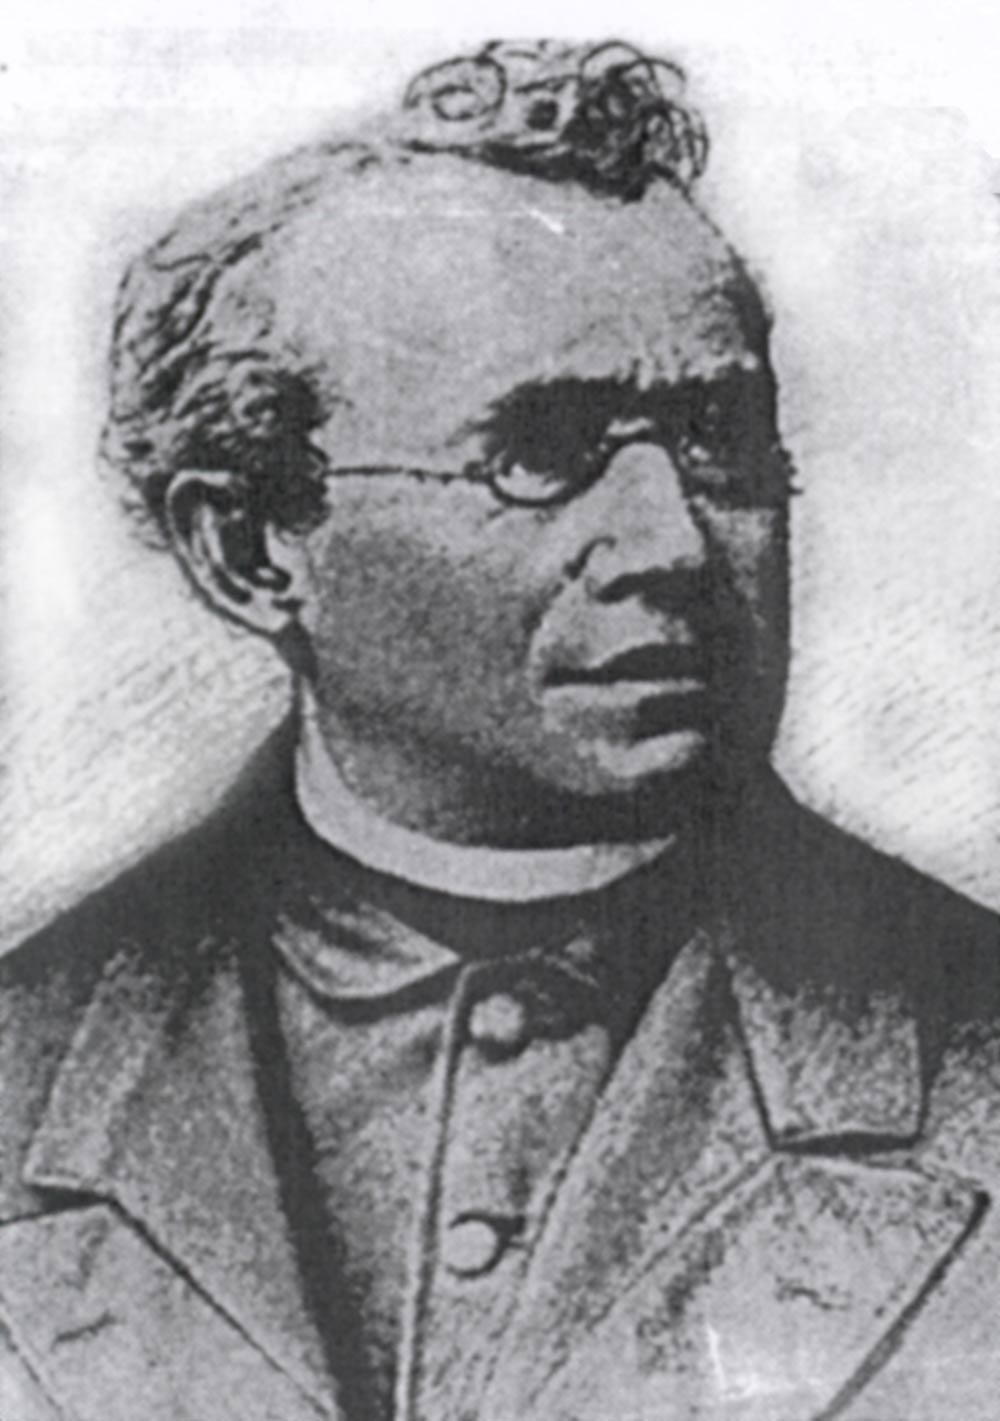
\includegraphics[width=3.016cm,height=4.284cm]{pictures/zulassungsarbeit-img078.jpg}

Franz Xaver Witt &

\begin{figure}
\img{}
\caption{}
\end{figure}

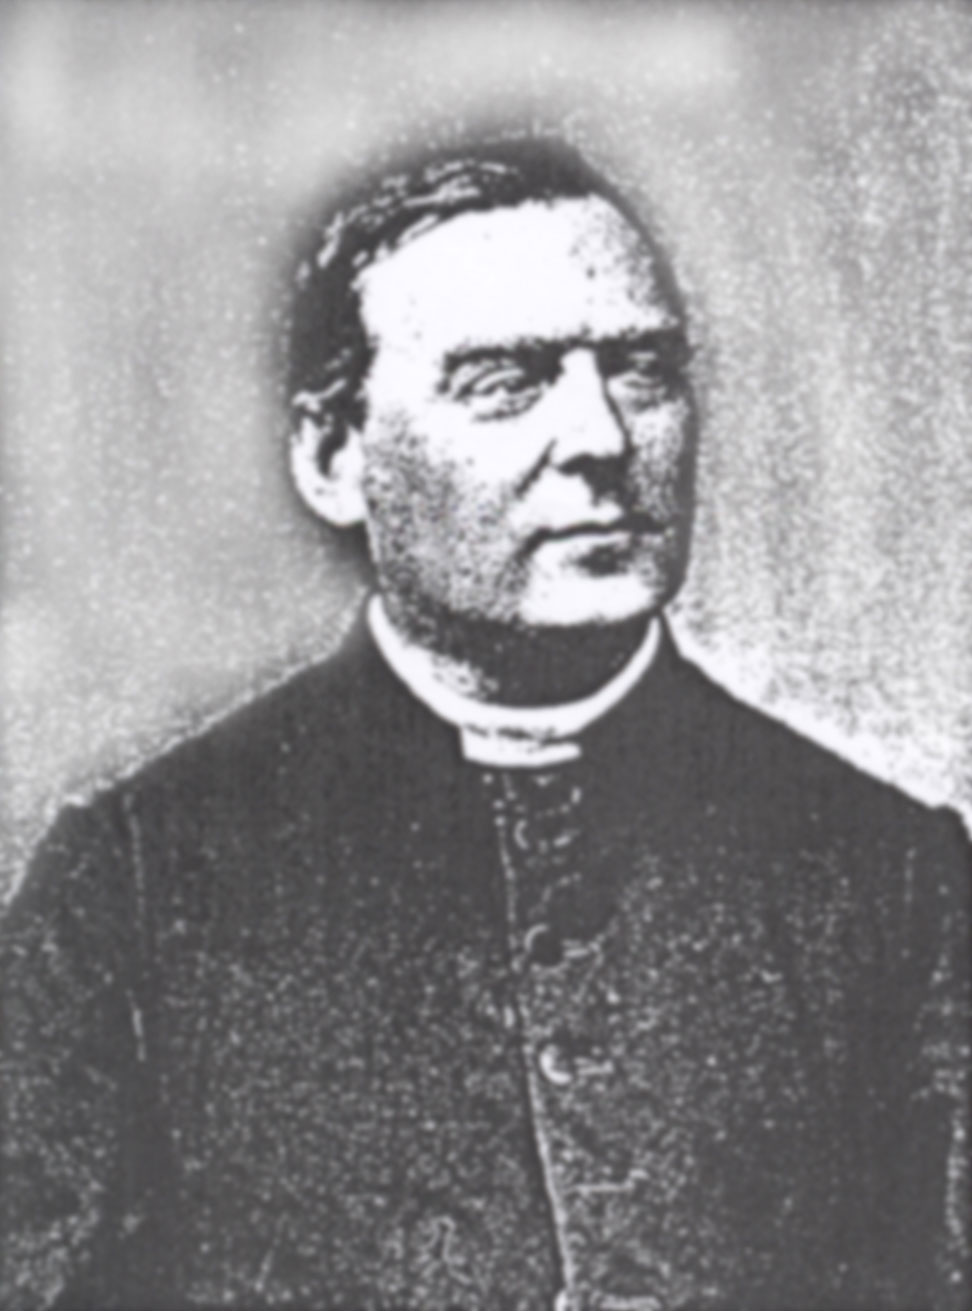
\includegraphics[width=3.163cm,height=4.3cm]{pictures/zulassungsarbeit-img079.jpg}

Franz Xaver Haberl\\
\end{supertabular}
\end{flushleft}
\end{minipage}
\end{center}

\begin{figure}
\img{}
\caption{}
\end{figure}

Die Motuproprio des damaligen Papstes “Inter pastoralis officii” im
Jahre 1903 bestätigt die Errungenschaften des Cäcilianismus auf der
einen Seite und stellt somit den Höhepunkt für die cäcilianische
Bewegung dar, leitete aber auf der anderen Seite das Ende der strengen
cäcilianistischen Periode ein, indem sie der \zitat{“modernen
Musik” } \footnote{Seidel, Seite 308} ihren eigenen Geltungsbereich in
der Kirchenmusik einräumte. Schon nach wenigen Jahrzehnten rigider
Orientierung am Palestrina-Ideal riss nicht nur der Bezug der
Kirchenmusik zu aktellen Strömungen der weltlichen Musik vollkommen ab,
sondern viele der im Geiste des Cäcilianismus erstandenen Kompositionen
verloren angesichts ihrer Anlage als reine Stilkopie jegliche Bedeutung
im Vergleich zu den kompositorischen Errungenschaften der damaligen
Gegenwart. Es ist deshalb den jüngeren Cäcilianern, wie etwa Peter
Griesbacher oder Vinzenz Goller, zu verdanken, dass sich der
Cäcilianismus weiter entwickelte und nicht im Historis-mus erstarrte.
Diese verstanden es nämlich, alte Stilelemte aus dem Cäcilianismus mit
Neuerungen des Zeitstils geschickt miteinander zu verbinden.\footnote{
Seidel, Seite 308} Dieser sich ab 1903 entwickelende Kirchenmusikstil
sei im folgenden “neuerer oder gemäßigter Cäcilianismus“ genannt. Der
Kirchenmusikstil seit Einsetzen der cäcilianischen Reformbewegung bis
1903 wird als “ursprünglicher, älterer oder strenger Cäcilianis-mus”
bezeichnet.

Beim Studieren des Notenbestands der Pfarrkirche St. Laurentius in
Ruhman-nsfelden kann dieser stilistische Übergang nachvollzogen werden.
Den alten strengen Cäcilianismus repräsentiert das meist noch
handschriftlich angefertigte Notenmaterial des Lehrer Max Weigs, der
von 1871 bis 1895 in Ruhmannsfelden Chorregent war. Dieser hat unter
anderem auch Werke von Franz Xaver Witt, einem Cäcilianer der ersten
Stunden, abgeschrieben. Die Werke, die August Högn nachweislich als
Chorregent aufgeführt hat, – er hinterließ an ihnen Spuren wie
Eintragungen, seinen Namenstempel, handschriftliche Abschriften oder
von ihm beschriftete Umschläge (siehe Band II, Seite 99) – sind
abgesehen von wenigen Ausnahmen stilistisch dem neuerem, gemäßigten
Cäcilianismus zuzuordnen. Allein die Tatsache, dass August Högn den
Großteil von Weigs Aufführungsmaterial vernichtet hat, indem er das
Notenpapier für seine Abschriften, Arrangements und Kompositionen
wieder verwendete, zeigt, dass zumindest ab 1920 als Högn zum ersten
Mal Chorregent wurde, Kompositionen im frühen, strengen cäcilianischen
Stil als unmodern galten.

Die Beeinflussung Högns eigenes musikalisches Schaffen, insbesondere die
der zur Chorregentenzeit Högns entstandenen Stücke, durch sein
kirchenmusikalisches Repertoire (neuerer Cäcilianimus) wird im Kapitel
 näher erläutert. Bei einigen seiner Kompositionen
orientierte er sich so stark an bereits vorhandene Werke aus seinem
Repertoire, sodass ein Werk entstand, das an manchen Passagen an ein
Plagiat erinnert. Eine derartige Arbeitsweise unterstreicht die
stilistische Beeinflus-sung seiner eigenen Kompositionen durch die von
ihm aufgeführten Werke und damit den großen Einfluss des gemäßigten
Cäcilianismus auf sein kirchenmusik-alisches Schaffen.